\documentclass[a5paper,12pt]{article}

\usepackage[utf8]{inputenc}
\usepackage{fontenc}
\usepackage[czech]{babel}

\usepackage{amsmath}
\usepackage{amsfonts}
\usepackage{mathtools}
\usepackage{enumitem}
\usepackage{multicol}

\usepackage{graphicx}
\usepackage[margin=1.5cm]{geometry}
\usepackage{color}
\PassOptionsToPackage{hyphens}{url}\usepackage[dvips]{hyperref}

\author{
  René Kliment 
  ( \href{mailto:klimeren@fjfi.cvut.cz}{klimeren@fjfi.cvut.cz} )
}
\title{TEF2 Cheatsheet}
\date{Kompilace dokumentu: \today}

\begin{document}

\maketitle
\tableofcontents

\newpage

% \begin{abstract}
% some info
% \end{abstract}

\section{Základní definice pravdy - L a H}

\subsection*{Obecné tipy}
\begin{itemize}
 \item dávat pozor na to, kde se sumuje, i když není napsaný znak sumy (Einsteinova sumace)
\end{itemize}


\subsection{Lagrangián}

\begin{equation*}
	\boldsymbol{L=L(q_i, \dot{q}_i, t) = T - U}
\end{equation*}

\begin{itemize}
	\item Eulerova-Lagrangeova rovnice: $\frac{d}{dt} (\frac{\partial L}{\partial \dot{q}_i}) - \frac{\partial L}{\partial q_i} = 0$\\
	$\qquad i \in \hat{s}$, kde $s$ je počet stupňů volnosti
	\item obecná hybnost: $p_j \coloneqq \frac{\partial L}{\partial \dot{q}_j}$
	\item obecná energie $E \coloneqq \sum_{j} \frac{\partial L}{\partial \dot{q}_j}\dot{q}_j - L$
	\item LHO: $L(x, \dot{x}) = \frac{1}{2}m\dot{x}^2 - \frac{1}{2}kx^2$
	\item EM pole $\varphi(\vec{r}, t), A(\vec{r}, t): \quad L = \frac{1}{2}m\vec{v}^2 - e(\varphi - \vec{v} \cdot \vec{A})$
\end{itemize}

\subsection{Hamiltonián}

\begin{equation*}
	\boldsymbol{H=H(q_i, p_i, t)}
\end{equation*}

Tohle najdeme a dosadíme dolů ${\color{red} \dot{q}_i} = f_i(q_j, p_j, t)$
\begin{equation*}
	H = H(q_i, p_i, t) \coloneqq \sum^{s}_{i=1} p_i {\color{red} \dot{q}_i} - L(q_i, {\color{red} \dot{q}_i}, t) = E(q_i, {\color{red} \dot{q}_i}, t)
\end{equation*}

\begin{equation*}
\boxed{
	\dot{q}_j = \frac{\partial H}{\partial p_j}
}
	\qquad j \in \hat{s} \qquad
\boxed{
	\dot{p}_j = - \frac{\partial H}{\partial q_j} 
}
\end{equation*}

\begin{itemize}
	\item $\frac{\partial H}{\partial t} = - \frac{\partial L}{\partial t}$
	\item LHO: $H(x, p) = \frac{p^2}{2m} + \frac{1}{2}kx^2$ \qquad
	$\dot{x} = \frac{p}{m}$ \qquad
	$\dot{p} = -kx$
	\item 1D EM pole $\varphi(r, t), A(r, t): \quad H = \frac{1}{2m}(p - eA)^2 + e\varphi$
	
\end{itemize}

\subsection{Populární L\&H}

\subsubsection{Volný hmotný bod v konzervativním poli}
\begin{itemize}
	\item sférické souřadnice\\
	\begin{flalign*}
	 L &= \frac{1}{2}m(\dot{r}^2 + r^2 \dot{\theta}^2 + r^2 sin^2(\theta \dot{\varphi}^2)) - U(r, \theta, \varphi)\\
	 H &= \frac{1}{2m}(p_r^2 + \frac{p_\theta^2}{r^2} + \frac{p_\varphi^2}{r^2 sin^2\theta}) + U(r, \theta, \varphi)
	\end{flalign*}
	
	\item cylindrické souřadnice\\
	\begin{flalign*}
	 L &= \frac{1}{2}m(\dot{r}^2 + r^2 \dot{\varphi}^2 + \dot{z}^2) - U(r, \varphi, z)\\
	 H &= \frac{1}{2m}(p_r^2 + \frac{p_\varphi^2}{r^2} + p_z^2) + U(r, \varphi, z)
	\end{flalign*}
	
\end{itemize}

\section{Integrály pohybu}

\subsection{Poissonova závorka}

\begin{equation*}
	\{F, G\} \coloneqq \sum_{i=1}^s \frac{\partial F}{\partial q_i}\frac{\partial G}{\partial p_i} - \frac{\partial F}{\partial p_i}\frac{\partial G}{\partial q_i}
\end{equation*}

\begin{enumerate}
	\item je antisymetrická $\boldsymbol{\{F, G\} = - \{G, F\}} \implies \{F, F\} = 0$
	\item je bilineární $\boldsymbol{\{cF_1 + F_2, G\} = c\{F_1, G\} + \{F_2, G\}}$\\ 
		\textit{(a také pro druhý argument)}
	\item Jacobiho identita\\ 
		$\boldsymbol{\{F_1, \{F_2, F_3\}\} + \{F_2, \{F_3, F_1\}\} + \{F_3, \{F_1, F_2\}\} = 0}$\\ 
		\textit{(tip: ty čísla jsou sudé permutace (1 2 3))}
	\item $\boldsymbol{\{F_1 F_2; G\} = F_1\{F_2; G\} + \{F_1; G\}F_2}$
	\item $\boldsymbol{\frac{\partial}{\partial t} \{F, G\} = \{\frac{\partial F}{\partial t}, G\} + \{F, \frac{\partial G}{\partial t}\}}$
\end{enumerate}

\subsection{Populární Poissonovy závorky}

\begin{itemize}
	\item $\{q_i, q_j\} = 0 = \{p_i, p_j\}$
	\item $\{q_i, p_j\} = \delta_{ij}$
	\item $\{L_i, L_j\} = \varepsilon_{ijl}L_l \qquad$ kde $\qquad L_i = \varepsilon_{ikl}x_k p_l$
	\item $\{L_i, p_j\} = \varepsilon_{ijl}p_l$
	\item $\dot{q}_i = \{q_i, H\}$ $\quad\qquad$ $\dot{p}_i = \{p_i, H\}$
\end{itemize}

\subsection{Integrály pohybu (= zachovávající se veličiny)}

\begin{itemize}
	\item definice: $F=F(q_i, p_i, t)$ je IP ${\iff} F(q_i(t), p_i(t), t) = const \quad \forall t$
	\item Věta: F je IP ${\iff} \boxed{\frac{dF}{dt} = \{F, H\} + \frac{\partial F}{\partial t} = 0}$
	\item cyklické souřadnice\\ \\
		$\frac{\partial H}{\partial q_i} = 0 \implies p_i$ je IP\\
		$\frac{\partial H}{\partial p_i} = 0 \implies q_i$ je IP\\
	\item Hamiltonián: $\frac{\partial H}{\partial t} = 0 \implies H$ je IP
	\item Věta (Poissonova): $F_1, F_2$ jsou IP $\implies \{F_1, F_2\}$ je IP
		
\end{itemize}

\newpage

\section{Kánonické transformace}

\subsection{Odkud kam}

\begin{flalign*}
	(q_i, p_i) &\rightarrow (Q_i, P_i)\\
	Q_i &= Q_i (q_j, p_j, t)\\
	P_i &= P_i (q_j, p_j, t)\\
	H(q_j, p_j, t) &\rightarrow H'(Q_i, P_i, t)
\end{flalign*}

Tato transformace je kánonická ${\iff}$ současně platí I. a II. sady Hamiltonových rovnic jak pro všechna $q_k, p_k$ pro $H$, tak $Q_k, P_k$ a $H'$.

\subsection{Vytvořující funkce}

\begin{enumerate}
\item $\boldsymbol{F_1 = F_1(q_j, Q_k, t)}$\\
\begin{equation*}
\boxed{
p_j = \frac{\partial F_1}{\partial q_j} \qquad
P_k = - \frac{\partial F_1}{\partial Q_k} \qquad
H' = H + \frac{\partial F_1}{\partial t}
}
\end{equation*}

\item $\boldsymbol{F_2 = F_2(q_j, P_k, t)}$\\
\begin{equation*}
\boxed{
p_j = \frac{\partial F_2}{\partial q_j} \qquad
Q_k = \frac{\partial F_2}{\partial P_k} \qquad
H' = H + \frac{\partial F_2}{\partial t}
}
\end{equation*}
\end{enumerate}

\subsection{Jak najít $F_i$ ?}

\begin{enumerate}
	\item pokud transformace nezávisí na $t$, ani $F_i$ nezávisí na t
	\item chci-li $\boldsymbol{F_1}$, pak musím najít $\boldsymbol{p_j (q_i, Q_i)}$ a $\boldsymbol{P_k (q_i, Q_i)}$ ... pokud to nejde (neumím vyjádřit v příslušných proměnných), tak hledám $\boldsymbol{F_2}$ tak, že se snažím najít $\boldsymbol{p_j = p_j (q_i, P_i)}$ a $\boldsymbol{Q_k = Q_k (q_i, P_i)}$
	\item pokud nejde ani jedno, tak mám asi smůlu
\end{enumerate}

\subsection{Ověření kánoničnosti transformace pomocí Poissonových závorek}
Pokud $\frac{\partial F_i}{\partial t} = 0$ a jsou splněny zároveň následující vztahy:
\begin{enumerate}
	\item $\{Q_i, P_j\} = \delta_{ij}$
	\item $\{Q_i, Q_j\} = 0$
	\item $\{P_i, P_j\} = 0$
\end{enumerate}

\noindent pak je transformace kánonická.

\newpage

\section{Hamiltonova-Jacobiho rovnice}

\begin{itemize}[leftmargin=*]

\item 
hledáme $F_2 = F_2(q_i, P_k, t)$ tak, aby $H' = 0$\\

$H' = H(q_i, p_i, t) + \frac{\partial F_2}{\partial t} = 0 \qquad {\color{red} p_i = \frac{\partial F_2}{\partial q_i}}$

\begin{equation*}
\boxed{
	H(q_i, {\color{red} \frac{\partial F_2}{\partial q_i}}, t) + \frac{\partial F_2}{\partial t} = 0
}
\end{equation*}

\item řešení závisí na $s+1$ konstantách, z nichž jedna je aditivní, takže ji ignorujeme $\rightarrow s$ konstant ($P_1,...,P_s$) $\implies \dot{P}_i = \frac{\partial H'}{\partial Q_i} = 0$\\

\item Řešení HJR, $S = S(q_i, P_k, t)$ nazýváme \textit{Hlavní funkcí Hamiltonovou}.

\begin{equation*}
H' = H + \frac{\partial S}{\partial t} = 0 \implies H = -\frac{\partial S}{\partial t}
\end{equation*}

\item $S$ je vytvořující funkcí 2. druhu ($F_2$), tedy:
\begin{equation*}
p_i = \frac{\partial S}{\partial q_i}(q_j, P_k, t) \qquad
Q_i = \frac{\partial S}{\partial P_i}(q_j, P_k, t) 
\end{equation*}

\item $P_k = const$, $Q_k = const \impliedby H' = 0$ (+ Hamiltonovy rovnice)

\item smysl \textit{HFH}: 
\begin{equation*}
\frac{d S}{d t} = L 
\end{equation*}
\textit{HFH} je akce vypočtená podél skutečné trajektorie
\begin{equation*}
S = \int_{t_0(Q_j)}^{t(q_j)} L dt
\end{equation*}

\end{itemize}
Užitečné externí linky:\\
\url{http://fyzika.jreichl.com/main.article/view/1290-hamiltonova-jacobiho-rovnice} \\
\url{http://fyzika.jreichl.com/main.article/view/1291-postup-reseni-hamiltonovy-jacobiho-rovnice}

\section{Integrabilní soustavy}

Soustava s $s$ stupni volnosti a Hamiltoniánem $H=H(q_i,p_i)$ je integrabilní, pokud existuje $s$ globálních nezávislých integrálů pohybu $P_j = P_j(q_i, p_i)$ v involuci, tj.:
\begin{enumerate}
	\item $\{P_j, H\} = 0 \qquad j \in \hat{s}$
	\item $\{P_j, P_k\} = 0 \qquad j,k \in \hat{s}$
	\item $(\nabla P_j)_{j=1}^{s}$ jsou LN\\ 
	na $M = \{(q_i, p_i) | P_j(q_i, p_i) = \alpha_j (const.) \forall j \in \hat{s} \}$
\end{enumerate}

\noindent kde $\nabla P_j = (\frac{\partial P_j}{\partial q_1}, ..., \frac{\partial P_j}{\partial q_s}, \frac{\partial P_j}{\partial p_1}, ..., \frac{\partial P_j}{\partial p_s})$

\section{Speciální teorie relativity}

Vycházíme ze 2 principů:
\begin{enumerate}
	\item princip relativity
	\item princip konstantní rychlosti světla $c$
\end{enumerate}

\subsection{Vztažné soustavy}

\begin{figure}[h!]
	\centering
	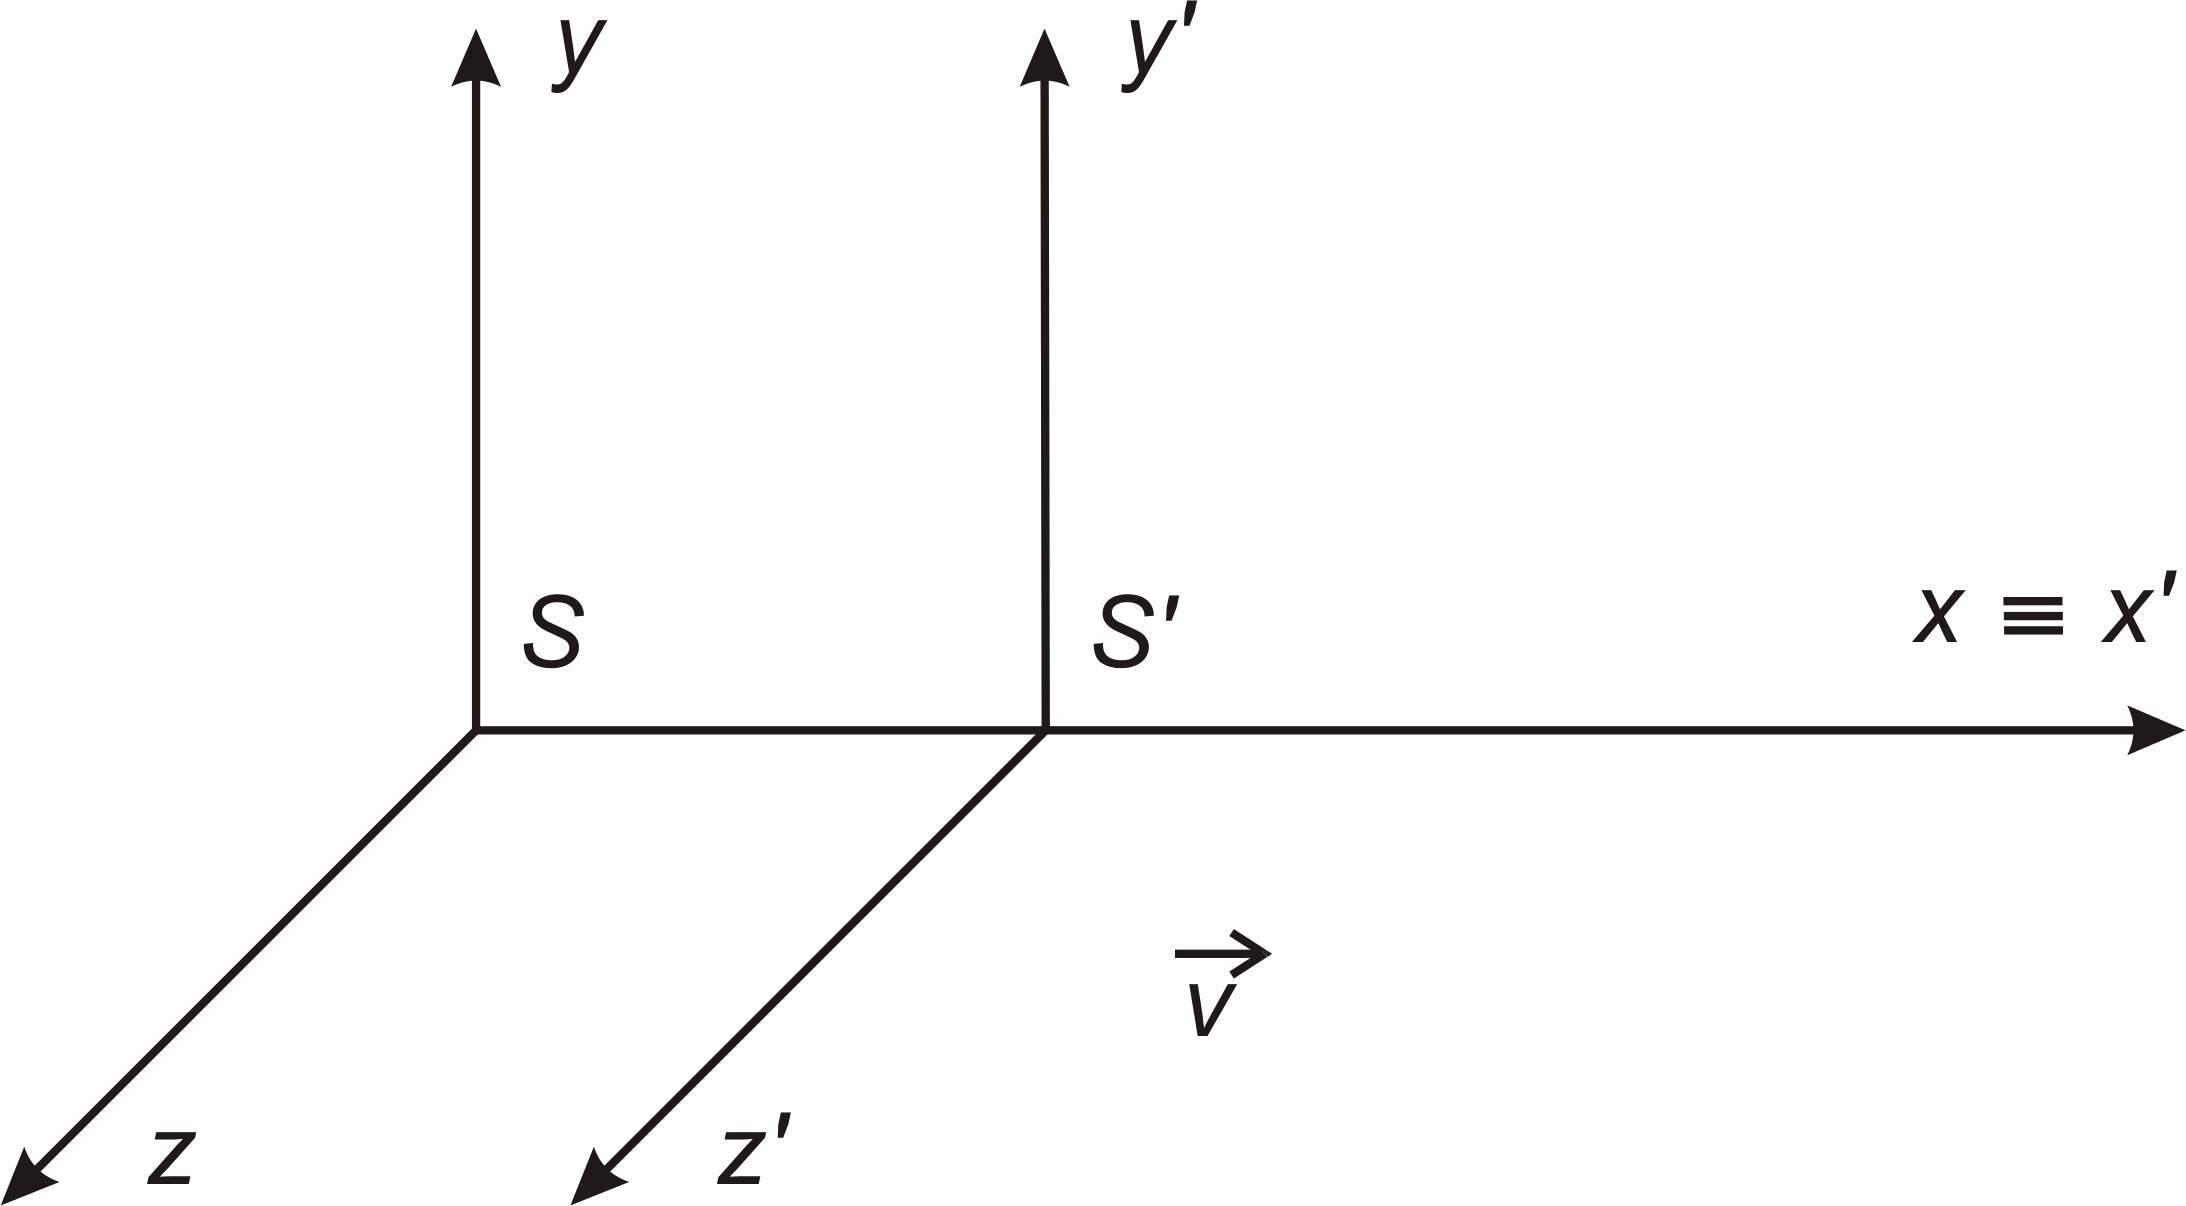
\includegraphics[width=0.5\textwidth]{data/Vztazna_soustava.png}
	\caption{Vztažné soustavy - soustava $S'$ se pohybuje ve směru $x$ rychlostí $V$ vůči soustavě $S$; Autor: \url{http://cs.wikipedia.org/wiki/Wikipedista:Vitecek}}
\end{figure}

\subsection{Galileiho transformace}

\begin{multicols}{2}\noindent
\begin{align*}
	x' &= x - Vt\\
	y' &= y\\	
	z' &= z\\	
	t' &= t
\end{align*}
\columnbreak
\begin{align*}
	\dot{x}' &= \dot{x} - V\\
	\dot{y}' &= \dot{y}\\
	\dot{z}' &= \dot{z}
\end{align*}
\end{multicols}

\subsection{Speciální Lorentzovy transformace}

Pro zjednodušení si zavedeme:
\begin{equation*}
\beta = {V\over c}\,,		\qquad		\boldsymbol{\gamma = {1 \over \sqrt{1 - {V^2 \over c^2}}}} = {1 \over \sqrt{1-\beta^2}}
\end{equation*}

\noindent Lorentzovy transformace pak můžeme napsat takto:

\begin{multicols}{2}\noindent
\begin{align*}
x^\prime &= \frac{x - Vt}{\sqrt{1 - \frac{V^2}{c^2}}} = \gamma\left(x - Vt\right) \\
y^\prime &= y\\
z^\prime &= z\\
t^\prime &= \frac{t - \frac{Vx}{c^2}}{\sqrt{1 - \frac{V^2}{c^2}}} =  \gamma\left(t - \frac{Vx}{c^2}\right)
\end{align*}
\columnbreak
\begin{align*}
x &= \frac{x^\prime + Vt^\prime}{\sqrt{1 - \frac{V^2}{c^2}}}\\
y &= y^\prime\\
z &= z^\prime\\
t &= \frac{t^\prime + \frac{Vx^\prime}{c^2}}{\sqrt{1 - \frac{V^2}{c^2}}}
\end{align*}
\end{multicols}

\textbf{Inverzní transformace} vznikne prohozením čárek/nečárek u souřadnic a změnou znaménka u $V$.\\

\noindent Maticově:
\begin{equation*}
	\begin{bmatrix}c t' \\ x' \\ y' \\ z'\end{bmatrix}
	=
	\begin{bmatrix}\gamma&-\beta \gamma&0&0\\-\beta \gamma&\gamma&0&0\\0&0&1&0\\0&0&0&1\\\end{bmatrix}
	\begin{bmatrix}c\,t \\ x \\ y \\ z\end{bmatrix}
\end{equation*}

\begin{itemize}
	\item základní invariant - \textit{kvadrát intervalu} $s^2$
	\begin{align*}
	s^2 &= x^2 + y^2 + z^2 - (ct)^2\\
	s'^2 &= x'^2 + y'^2 + z'^2 - (ct')^2
	\end{align*}

	\item Minkowski značí $x^0 = ct \qquad x^1 = x \qquad x^2 = y \qquad x^3 = z$
	
	\item světelné vlnoplochy $s'^2 = s^2 = 0$
	
	\item dilatace času $\boldsymbol{dt = \gamma d\tau}$
	
	\item kontrakce délek $\boldsymbol{l = \gamma{}^{-1} l_0}$
	
	\item skládání rychlostí $\boldsymbol{v' = \frac{v - V}{1 - \frac{Vv}{c^2}}}$
	
\end{itemize}

\subsection{Čtyřveličiny}

\begin{itemize}
	\item čtyřrychlost 
	\begin{equation*}
		(u^\mu) = \left(\frac{c}{\sqrt{1 - \frac{V^2}{c^2}}}, \frac{\vec{v}}{\sqrt{1 - \frac{V^2}{c^2}}}\right)
	\end{equation*}
	
	\item čtyřhybnost 
	\begin{equation*}
		(p^\mu) = \left(\frac{m_0 c}{\sqrt{1 - \frac{V^2}{c^2}}}, \frac{m_0 \vec{v}}{\sqrt{1 - \frac{V^2}{c^2}}}\right)
	\end{equation*}
	
	\item čtyřsíla
	\begin{equation*}
		K^{\mu} = \frac{d p^{\mu}}{d \tau} 
	\end{equation*}

\end{itemize}


\end{document}